\documentclass[handout,t,compress]{beamer}
\usepackage{etex}
\usetheme{Singapore}

\sloppy
%\usepackage[scaled]{helvet}
%\usepackage{eulervm}

\usepackage{fp-eval}
\usepackage{hyperref}
\usepackage{fancyvrb}
\usepackage{multicol}
\usepackage{pstricks,pst-node,pst-tree,pst-plot,pst-3dplot,multido}
\usepackage{graphicx}

\usepackage{alltt}

\newcommand{\bi}{\begin{itemize}}
\newcommand{\ii}{\item}
\newcommand{\ei}{\end{itemize}}

\newcommand{\bframe}[1]{\begin{frame}[fragile]{#1}}

\newcommand{\bbnf}{\begin{center}\begin{tabular}{rcl}}
\newcommand{\bnf}[2]{#1 & ::= & #2 \\}
\newcommand{\ebnf}{\end{tabular}\end{center}}

\newcommand{\myskip}{\vspace{-1em}\hrulefill}
\newcommand{\myrule}[1]{\vspace{-1ex}\centerline{\rule{#1cm}{1pt}}}
\newcommand{\myline}[1]{\centerline{#1}}
\newcommand{\bkt}[1]{\ensuremath{\langle\mbox{#1}\rangle}}
\newcommand{\br}{\mbox{~}|\mbox{~}}

\definecolor{orange}{rgb}{1,.5,0}
\definecolor{pink}{rgb}{1,.75,.75}
\definecolor{ltblue}{rgb}{.75,.75,1}

\newcommand{\be}{\begin{eqnarray*}}
\newcommand{\ee}{\end{eqnarray*}}

\newcommand{\grph}[2]{
\begin{columns}
\column{0.01\textwidth}
\column{0.6\textwidth}
\begin{pspicture}[showgrid=#1](-2,-2)(5,5)
#2
\end{pspicture}
}

\newcommand{\txt}[1]{
\column{0.4\textwidth}
\rput[bl](0,0){\parbox{\textwidth}{
\footnotesize
\begin{itemize}
#1
\end{itemize}}}
\end{columns}}

\newcommand{\myvec}[1]{
\pstThreeDDot[showpoints=true,drawCoor=true](#1)
\pstThreeDLine[arrows=->,linecolor=blue](0,0,0)(#1)
}

\AtBeginSection[]
{
\bframe{Outline}
\tableofcontents[currentsection]
\end{frame}
}

\title{Physics Notes \#3: Collisions}
\author{CSCI 321}
\institute{WWU}

\begin{document}\small
\psset{arrowscale=2}

\bframe{~}
\titlepage
\end{frame}

\bframe{Advanced collision techniques}

Reading:
\begin{itemize}
\item {\tiny
\url{http://www.gamasutra.com/view/feature/3429/crashing_into_the_new_year_.php}}
\item {\tiny
\url{http://www.gamasutra.com/view/feature/3426/when_two_hearts_collide_.php}}
\item {\tiny
\url{http://www.gamasutra.com/view/feature/3427/collision_response_bouncy_.php}}
\item {\tiny
\url{http://www.gamasutra.com/view/feature/3190/advanced_collision_detection_.php}
}

\end{itemize}

\end{frame}

\bframe{Is a point inside a polygon?}
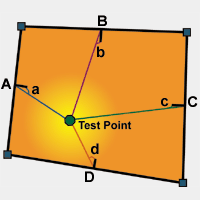
\includegraphics[scale=0.75]{Figures/lander01/lander_figure_01.png}
\bi
\ii Dot vector to point with inward pointing normal.
\ii Polygons usually have a consistent winding direction.
\ii How can you quickly find the inward pointing normal?
\ei
\end{frame}
\bframe{Does not work with concave polygons}
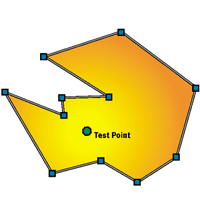
\includegraphics[scale=0.75]{Figures/lander01/lander_figure_02.png}
\end{frame}
\bframe{Sum of all the angles = 360?}
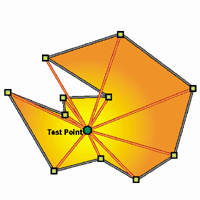
\includegraphics[scale=0.75]{Figures/lander01/lander_figure_03.png}
\end{frame}
\bframe{Quadrant crossing = 4?}
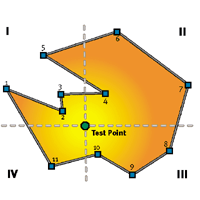
\includegraphics[scale=0.75]{Figures/lander01/lander_figure_04.png}

Or check even/odd intercepts.
\end{frame}
\bframe{Keeping at arm's length}
\begin{multicols}{2}
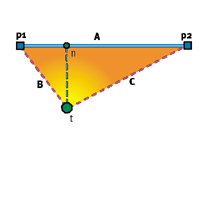
\includegraphics[scale=0.75]{Figures/lander01/lander_figure_05.png}

\columnbreak

\begin{eqnarray*}
A &=& p_2 - p_1\\
B &=& t - p_1\\
C &=& t - p_2\\
n &=& p_1 + A\frac{B\cdot A}{(B\cdot A) + (C \cdot A)}\\
\\
A_{norm} &=& \frac{A}{|A|}\\
n &=& p1 + A_{norm}(B\cdot A_{norm})
\end{eqnarray*}
\end{multicols}
\end{frame}
\bframe{Bounding spheres}
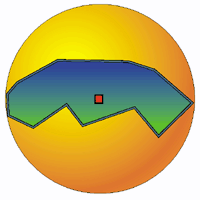
\includegraphics[scale=0.75]{Figures/lander01/lander_figure_06.png}
\bi
\ii Collision between spheres?
\ii Collision sphere with polygon?
\ei
\end{frame}
\bframe{Find a separating plane}
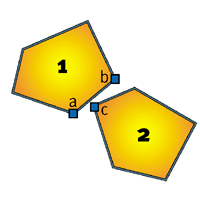
\includegraphics[scale=0.75]{Figures/lander01/lander_figure_07.png}
\bi
\ii See notes on Verlet integration:

\url{http://www.gamedev.net/page/resources/_/technical/math-and-physics/a-verlet-based-approach-for-2d-game-physics-r2714}
\ei
\end{frame}


\bframe{Axis-aligned bounding box (AABB)}
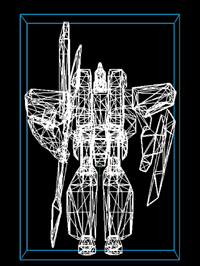
\includegraphics[scale=0.75]{Figures/lander02/lander_figure_01.png}
\hfill
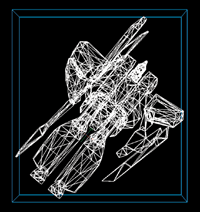
\includegraphics[scale=0.75]{Figures/lander02/lander_figure_02.png}
\end{frame}
\bframe{Oriented bounding box (OBB)}
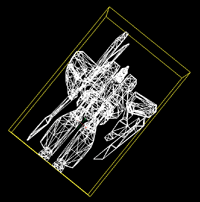
\includegraphics[scale=0.75]{Figures/lander02/lander_figure_03.png}
\end{frame}
\bframe{Fast and slow AABB calculation}
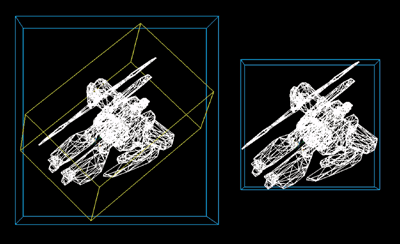
\includegraphics[scale=0.75]{Figures/lander02/lander_figure_04.png}
\end{frame}
\bframe{Two objects that might be colliding}
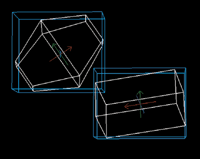
\includegraphics[scale=0.75]{Figures/lander02/lander_figure_05.png}
\end{frame}
\bframe{Find a separating plane:  first try faces}
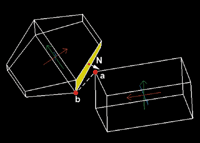
\includegraphics[scale=0.75]{Figures/lander02/lander_figure_06.png}
\end{frame}
\bframe{In 3D may not be a separating face}
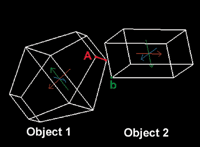
\includegraphics[scale=0.75]{Figures/lander02/lander_figure_07.png}

\bi\ii Need to check point-edge combinations as well.\ei
\end{frame}
\bframe{Other points}
\begin{itemize}
\item Cache separating planes.
\item Separating plane only works for convex objects.
\end{itemize}
\end{frame}

\bframe{Collision may happen between frames}
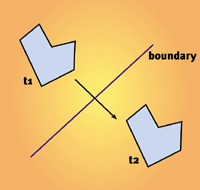
\includegraphics[scale=0.75]{Figures/bobic01/bobic_01.png}
\begin{itemize}
\item Smaller $\Delta t$ in the physics.
\item Don't make really thin walls.
\end{itemize}
\end{frame}
\bframe{Create convex hull from object in two different frames}
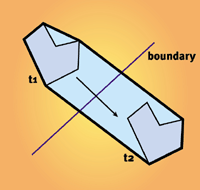
\includegraphics[scale=0.75]{Figures/bobic01/bobic_02.png}
\end{frame}
\bframe{Bounding spheres}
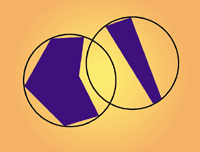
\includegraphics[scale=0.75]{Figures/bobic01/bobic_03.png}
\end{frame}
\bframe{Create tree of bounding spheres}
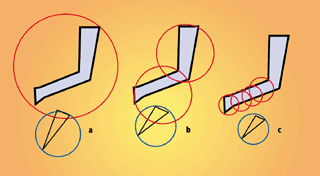
\includegraphics[scale=0.75]{Figures/bobic01/bobic_04.png}
\end{frame}
\bframe{AABB}
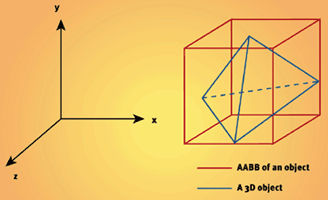
\includegraphics[scale=0.75]{Figures/bobic01/bobic_05.png}
\end{frame}
\bframe{AABBs for rotating objects}
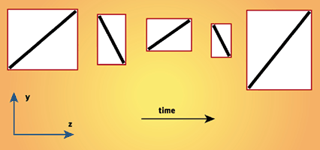
\includegraphics[scale=0.75]{Figures/bobic01/bobic_06.png}
\end{frame}
\bframe{Recursive OBB}
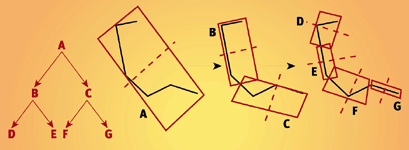
\includegraphics[scale=0.75]{Figures/bobic01/bobic_07.png}
\begin{itemize}
\item Check for collision at top level, if exists, recurse on both.
\item Note: Require artists to specify OBBs, convex hulls, {\em etc.}
  in advance.  
\end{itemize}
\end{frame}
\bframe{Check boxes for separating planes}
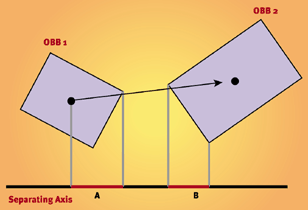
\includegraphics[scale=0.75]{Figures/bobic01/bobic_08.png}
\end{frame}
\bframe{Curved objects}
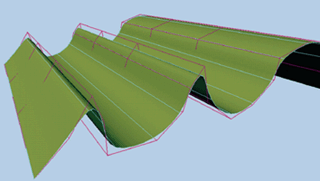
\includegraphics[scale=0.75]{Figures/bobic01/bobic_09.png}
\bi\ii Approximate with linear objects \ei
\end{frame}


\bframe{Minkowski sums}


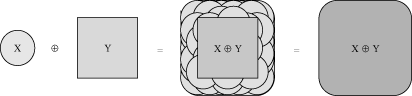
\includegraphics[scale=0.75]{IGD/MinkowskiSum01.png}

\bigskip

\hrulefill

\bigskip

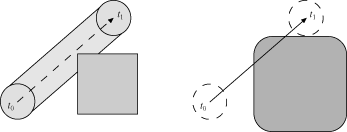
\includegraphics[scale=0.75]{IGD/MinkowskiSum02.png}
\end{frame}

\bframe{Complexity with many objects}
\[
\left(\begin{array}{c}N\\2\end{array}\right) = O(N^2)
\]

\end{frame}

\bframe{Partitioning: $O(N)$}
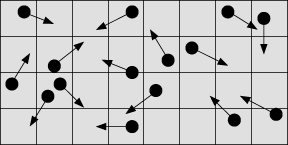
\includegraphics{IGD/Partition.png}
\end{frame}

\bframe{Sweep and prune: $O(N\log N)$}
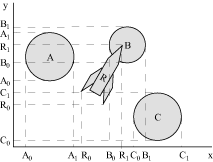
\includegraphics{IGD/SweepAndPrune.png}
\end{frame}



\bframe{Use a Library}
\begin{itemize}
\item \url{http://www.box2d.org/}
\item  \url{http://www.pymunk.org/}
\item \url{http://bulletphysics.org/}
\end{itemize}
\end{frame}

\end{document}
